\chapter{Theorie}
\label{cha:Theorie}


\section{Interferenzphänomene}
\label{sec:Interferenz}

Licht ist eine elektromagnetische transversale Welle und schwingt somit orthogonal zu seiner Ausbreitungsrichtung. Wenn
sich zwei sinusförmige elektromagnetische Wellen örtlich überlagern, kann sich je nach Phasenunterscheid und
Polarisationsrichtung eine
teilweise/gänzliche Verstärkung oder teilweise/gänzliche Auslöschung ergeben. Das nennt sich Interferenz.\\
Interferenzeffekte können grundsätzlich nur beobachtet werden, wenn diese zwei Wellen kohärent zueinander sind, also eine ähnliche
Frequenz aufweisen. In der Natur wird man nur schwer perfekt kohärente Wellen finden, da Licht selten monochromatisch ist, sondern
aus Wellenpaketen unterschiedlicher Frequenzen besteht. Allerdings kann man eine Kohärenzlänge identifizieren - ein räumlicher Abstand
in der Wellen als annähernd kohärent betrachtet werden können. Im folgenden ist anzunehmen, dass die miteinander interferierenden 
Wellen ausreichend kohärent zueinander sind.\\
Wenn ein Phasenunterscheid von
\begin{equation}
\label{eq:konstr}
    \delta = 2 \pi n, \, \. n \in \mathbb{N_0}
\end{equation}
vorliegt, addieren sich die Amplituden der Wellen konstruktiv. Bei einem Phasenunterscheid von
\begin{equation}
\label{eq:destr}
    \delta =  (2n+1)\pi, \, \. n \in \mathbb{N_0}
\end{equation}
interferieren Wellen destruktiv und löschen sich aus. Sofern die Werte zwischen diesen beiden Extremen liegen, findet
lediglich eine leichte Abschwächung oder Verstärkung der Amplitude statt.\\
Diese Interferenzeffekte lassen sich zusätzlich nur beobachten, sofern die zwei Wellen nicht linear unabhängig voneinander sind.
Das heißt, dass die Wellen nicht orthogonal zueinander schwingen dürfen. Eine maximale Auslöschung/Verstärkung kann nur bei gleicher
Polarisation beobachtet werden.\\
Die Polarisation einer elektromagnetischen Welle kann durch einen Polarisationsfilter überprüft werden, welcher je nach Ausrichtung 
nur eine Projektion der Welle auf diese Ebene durchlässt. Wenn Polarisationsrichtung des Filters und der Welle orthogonal aufeinander
stehen, kommt also Signal durch diesen Filter durch.\\

\section{Sagnac-Interferometer}
\label{sec:Sagnac}

Interferometer machen sich eben diese Eigenschaften von Wellen zur Nutze. Materialien weisen einen Brechungsindex aus, durch
welchen die Phase einer durchgehenden Welle manipuliert wird. Dies kann man sich zunutze machen, indem man einen unbeeinflussten Strahl und
einen manipulierten Strahl interferieren lässt und die Interferenzminima und -maxima untersucht. Auf diesem Wege lassen sich auch 
andere Materialeigenschaften untersuchen.\\
Im allgemeinen besteht ein Interferometer aus mehreren Spiegeln und Strahlteilern. In diesem Versuch wird das Sagnac-Interferometer untersucht,
welches in \autoref{fig:Aufbau} schematisch gezeigt ist.\\

\begin{figure}
    \centering
    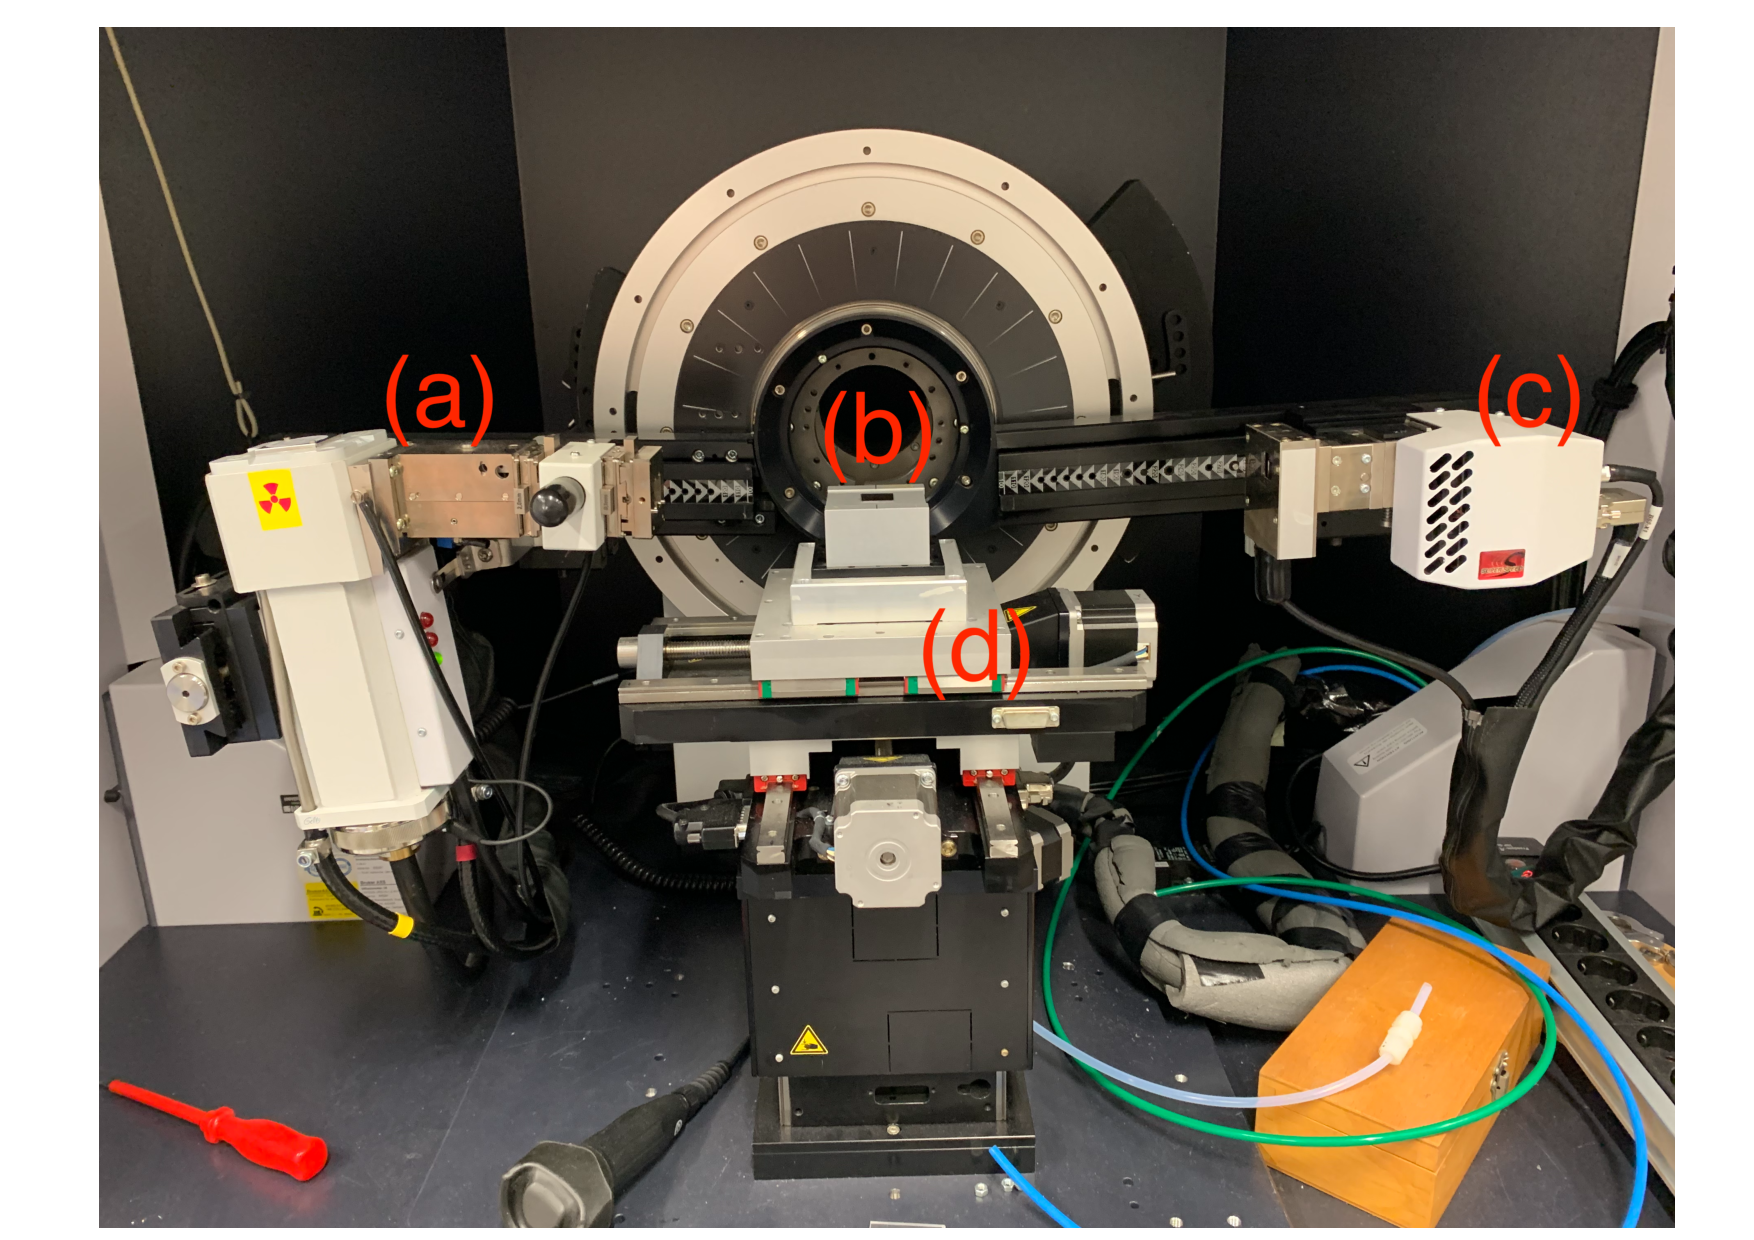
\includegraphics[scale=0.4]{content/V64_pictures/Aufbau.png}
    \caption{Eine schematische Darstellung eines Sagnac-Interferometers. \cite{v64}}
    \label{fig:Aufbau}
\end{figure}
Das Sagnac Interferometer besteht aus zwei Spiegeln (M1 und M2), welche den Laser in das eigentliche Interferometer ablenken. Dieser trifft dann 
zuerst auf einen Polarisationfilter mit Polarisationswinkel $phi$, sodass das Licht gleich linear polarisiert ist.\\
Dann trifft der Laserstrahl auf einen Strahlteilerwürfel (PBSC), welcher den Strahl in zwei orthogonal zueinander verlaufende Strahlen aufteilt. Diese Strahlen werden durch
den Würfel zudem orthogonal zueinander polarisiert. Der transmittierte Strahl wird parallel zur Einfallsebene und der reflektierte Strahl senkrecht
zur Einfallsebene polarisiert.\\
Die beiden Strahlen durchlaufen den Aufbau von drei Spiegeln nun genau entgegengesetzt und werden dann wieder durch den PBSC zusammengeführt. Dadurch, dass
die Strahlen denselben Weg durchlaufen, ist das Interferometer besonders stabil gegenüber Umwelteinflüssen, da diese auf beide Strahlen gleichermaßen wirken.\\
Um einen Strahl separat vom anderen manipulieren zu können, wird der Spiegel M2 parallel zum Aufbau verschoben, wodurch die Strahlen innerhalb des Interferometers einen
leicht anderen Weg verlaufen, aber am Ende vom PBSC wieder zusammengeführt werden. Mithilfe von einer (zwei) Diode\textit{n} kann die Spannung(sdifferenz) des Lasers
gemessen werden.

\section{Kontrast eines Interferometers}
\label{sec:Kontrast}
Die Qualität eines Interferometers kann durch seinen Kontrast/seine Sichtbarkeit beschrieben werden. Diese gibt wieder, wie deutlich sich die Intensität des
Interferenzmaximas und die des -minimas voneinander unterschieden. Er kann berechnet werden durch
\begin{equation}
    K = \frac{I_{max} - I_{min}}{I_{max} + I_{min}}.
\end{equation}
Um den Kontrast mithilfe dieser Formel berechnen zu können, muss die Intensität experimentell ermittelt werden. Um den Kontrast theoretisch vorhersagen
zu können, überlegt man zunächst, welche Proportionalität die resultierende Intensität gegenüber unserer einzelnen Wellen hat. Hier kommt man auf die Formel
\begin{equation}
    \label{eq:prop}
    I \propto \langle \mid E_1 \cos{(\omega t)} + E_2 \cos{(\omega t + \delta)} \mid^2 \rangle,
\end{equation}
wobei $E_1$ und $E_2$ die Amplituden der einzelnen Wellen, $\omega$ die Kreisfrequenz und $\delta$ der Phasenunterscheid ist. $\langle ... \rangle$ ist das zeitliche Mittel.
Durch den Polarisationfilter und PBSC gilt
für die einzelnen Amplituden der Wellen
\begin{equation}
    E_1 = E_0 cos{(\phi)}
\end{equation}
und
\begin{equation}
    E_2 = E_0 sin{(\phi)},
\end{equation}
wobei $E_0$ die Gesamtamplitude der einlaufenden Welle ist. Eingsetzt in \autoref{eq:prop} ergibt das
\begin{align}
    I   \propto& \langle \mid E_0 cos{(\phi)} \cos{(\omega t)} + E_0 sin{(\phi)} \cos{(\omega t + \delta)} \mid^2 \rangle \\
        \propto& E_0^2 \langle \left(\mid cos^2{(\phi)} \cos^2{(\omega t)} +  2 cos{(\phi)} \cos{(\omega t)} sin{(\phi)} \cos{(\omega t + \delta)} +  sin^2{(\phi)} \cos^2{(\omega t + \delta)} \mid \right) \rangle.
\end{align}
Die Maxima und Minima ergeben sich wie in \autoref{eq:konstr} und \autoref{eq:destr} erwähnt:
\begin{align}
    I_{max} \propto&  \langle E_0^2 \left(\mid cos^2{(\phi)} \cos^2{(\omega t)} +  2 cos{(\phi)} \cos{(\omega t)} sin{(\phi)} \cos{(\omega t + 2 \pi n)} +  sin^2{(\phi)} \cos^2{(\omega t + 2 \pi n)} \mid \right) \rangle  \\
            \propto&  \langle E_0^2 \left(\mid cos^2{(\phi)} \cos^2{(\omega t)} +  2 cos{(\phi)} \cos{(\omega t)} sin{(\phi)} \cos{(\omega t)} +  sin^2{(\phi)} \cos^2{(\omega t)} \mid \right) \rangle \\
            \propto&  \langle E_0^2 \cos^2{(\omega t)} \left(\mid cos^2{(\phi)} +  2 cos{(\phi)}sin{(\phi)} +  sin^2{(\phi)} \mid \right) \rangle,
\end{align}
wobei der Betrag des zeitlichen Mittels von $\cos^2{(\omega t)} = \frac{1}{2}$ und $cos^2{(\phi)} + sin^2{(\phi)} = 1$ ist. Somit ergibt sich
\begin{equation}
    I_{max} \propto I_{Laser} \left( 1 + 2 cos{(\phi)}sin{(\phi)} \right).
\end{equation}
$I_{Laser} = \frac{1}{2} E_0^2$ ist hier die mittlere Ausgangsintensität des Lasers.\\
Durch den gleichen Weg ergibt sich für die destruktive Interferenz
\begin{equation}
    I_{min} \propto I_{Laser} \left( 1 - 2 cos{(\phi)}sin{(\phi)} \right),
\end{equation}
da $\cos{(\omega t + (2n+1)\pi)} = -\cos{(\omega t)} $.\\
Anhand dieser Gleichungen ist bei jedem vielfachen von $\frac{\pi}{2}$ ein maximaler Kontrast zu erwarten.\\
Die Theoriekurve hierzu ist in \autoref{fig:Kontrast} zu sehen.
 
\begin{figure}
    \centering
    \includegraphics[scale=0.4]{content/V64_pictures/Kontrast.png}
    \caption{Der funktionelle Verlauf der Intensitäten(grün: $I_{max}$, blau: $I_{min}$) und des Kontrastes (rot).}
    \label{fig:Kontrast}
\end{figure}

\section{Brechungsindex von Glas}
\label{sec:BrechungGlas}
Mit Interferometern kann unteranderem wie bereits erwähnt der Brechungsindex von Materialien untersucht werden. Wenn sich eine elektromagnetische
Welle durch ein Material bewegt, verändert sich die Ausbreitungsgeschwindigkeit gemäß des Brechungsindexes $n$ und somit unwillkürlich auch der Wellenvektor $k$
der Welle.
\begin{equation}
    v_{Medium} = \frac{c}{n} \Rightarrow k = \frac{2\pi}{\lambda_{vac}}n,
\end{equation}
Die Strahlen werden hier jeweils durch ein um $\Theta = \pm 10^\circ$ rotiertes Glasplätchen geschickt. Hier findet einerseits eine Phasenverschiebung durch den Brechungsindex
und andererseits eine Phasenverschiebung durch die Lichtbrechung an dem Glasplätchen statt. Mit dem Brechungsgesetz nach Snellius und einer Taylorentwicklung für kleine
Winkel ergibt sich 
\begin{equation}
    \label{eq:Phi}
    \Delta \Phi = \frac{2\pi}{\lambda_{vac}}L\frac{n-1}{2n} \left((\Theta+Theta_0)^2 - (\Theta-\Theta_0)^2 \right).
\end{equation}
$L$ ist die Dicke des Mediums, $\lambda_{vac}$ die Wellenlänge im Vakuum, $c$ die Lichtgeschwindigkeit und $Delta \Phi$ die Phasenverschiebung.\\
Hier wird außerdem berücksichtigt, dass die Glasplätchen einen Winkel von $\Theta_0 = \pm 10^\circ$ zueinander haben.\\
Mithilfe einer Diode und eines Modern Interferometry Controller \cite{v64} können die Anzahl der Maxima mit
\begin{align}
\label{eq:Maxima}
    M   &= \frac{\Delta\Phi}{2\pi} \Leftrightarrow \Delta\Phi = 2M\pi  \\
        &\Rightarrow  \frac{M\lambda_{vac}}{L \left((\Theta+Theta_0)^2 - (\Theta-\Theta_0)^2 \right)} = \frac{n-1}{n} \\
        &n = \frac{1}{1- \frac{M \lambda_{vac}}{2 T \Theta \Theta_0}} 
\end{align}
berechnet werden. Das wird dann in \autoref{eq:Phi} eingesetzt und nach $n$ umgestellt.\\


\section{Brechungsindex von Gasen}
\label{sec:BrechungGas}

Die Phasenverschiebung in Gases funktioniert nach demselben Prinzip, allerdings hat hier lediglich den Einfluss des Brechungsindexes und nicht mehr zusätzlich
den Einfluss der geometrischen Brechung.
Dadurch findet eine Phasenverschiebung gegenüber des unbeeinflussten Strahls statt. Diese Phasendifferenz berechnet sich zu 
\begin{equation}
    \Delta \Phi = \frac{2\pi}{\lambda_{vac}}(n-1)L,
\end{equation}
mit der Dicke $L$ des Mediums. Die Phasenverschiebung kann wieder über die Maximaanzahl ausgedrückt werden nach \autoref{eq:Maxima}:
\begin{equation}
    n = \frac{M \lambda_{vac}}{L} + 1.
\end{equation}
Mit dem Lorentz-Lorenz-Gesetz lässt sich der Brechungsindex zudem über die Polarisierbarkeit des Mediums bestimmen:
\begin{equation}
    \frac{n^2-1}{n^2+1} = \frac{A p}{R T},
\end{equation}
wobei $A$ die Molrefraction, $p$ der Druck, $R$ die Gaskonstante und $T$ die Raumtemperatur ist. Dies lässt sich mit einer Taylorentwicklung 
um $n=1$ herum zu 
\begin{equation}
    n = \frac{3}{2} \frac{A p}{R T} + 1
\end{equation}
umformen. Diese Umformung ist in diesem Fall gültig, da Luft untersucht wird und $n_{Luft} \approx 1$.

